\problemname{Garbled Garden}

\newcommand{\maxn}{5000}

After an extremely tiring day at work, Tessa arrived home to find her husband waiting proudly at the door.
With a huge smile on his face, he announced that he had planted all her flowers in the garden.
Grateful that her husband had taken some work off her shoulders, she went straight out to the garden.
Her relief lasted exactly until she reached it.

While he did indeed manage to plant all of her flowers around the edge of the garden, unfortunately, the arrangement was very wrong.
Roses stood where the orchids should have been.
Hyacinths, dahlias, and chrysanthemums were scattered among the hydrangeas.
The whole garden looked as though a toddler had planted them.

Tessa stared at the numbered tags still tied to the stems.
She had arduously labelled every single flower with non-decreasing labels from left to right of the intended order.
Flowers of the same species had matching tags since the order within one type of flower did not matter.

Her husband followed her gaze to the labels, shrugged, and said he thought that they were price tags and had not paid any attention to them~\dots

\begin{figure}[h]
    \centering
    
\includegraphics[width=0.45\textwidth]{figure1}
    
\includegraphics[width=0.45\textwidth]{figure2}
\end{figure}
\vspace{-0.5cm}
\begin{figure}[h]
    \centering
    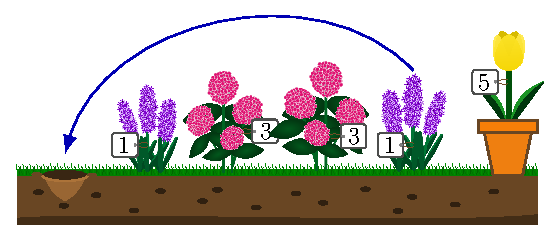
\includegraphics[width=0.45\textwidth]{figure3}
    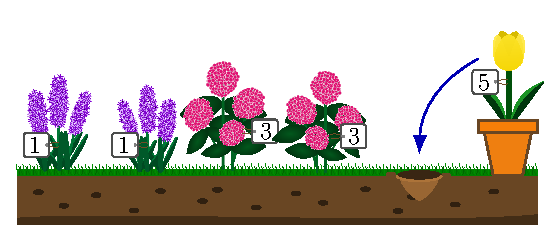
\includegraphics[width=0.45\textwidth]{figure4}
    \caption{Visualization of the second sample answer.}
\end{figure}

Sighing, she settled down and decided to fix this mess.
Since the flowers were still very young and delicate, she cannot just dig out some of the flowers, rearrange them, and then plant them back.
Instead, she can do the following operation:
\begin{itemize}
    \item She chooses an integer $m$ and a sequence of $m$ distinct integers $p_1, \dots, p_m$.
    \item First, she picks the flower at position $p_1$ and moves it back into a flowerpot.
    \item Then, she repeatedly chooses the flower at position $p_i$ ($i \geq 2$), and moves it to the now empty position $p_{i-1}$ of the previous flower.
    \item Finally, after $m-1$ iterations of the previous step, she finishes the operation by replanting the potted flower at the remaining empty position $p_m$.
\end{itemize}
Every flower can be used at most once within the \emph{same} operation due to their fragile nature.

Determine the minimum number of operations Tessa has to do to fix the arrangement, and output one possible sequence of these operations.

\newpage

\begin{Input}
    The input consists of:
    \begin{itemize}
        \item One line with an integer $n$ ($2 \leq n \leq \maxn$), the number of Tessa's flowers.
        \item One line with $n$ integers $t_1, \ldots, t_n$ ($1 \leq t_i \leq n$ for each $i$), where $t_i$ is the tag number of the flower at position $i$.
    \end{itemize}
\end{Input}

\begin{Output}
    First, output the minimum number of operations $k$ ($0 \leq k \leq n$) to fix the arrangement. It can be proven that there always is an answer taking at most $n$ operations.

    Then, for each of the $k$ operations, output:
    \begin{itemize}
      \item One integer $m$ ($1 \leq m \leq n$), the number of flowers moved in this operation.
      \item $m$ distinct integers $p_1, \ldots, p_m$ ($1 \leq p_i \leq n$ for each $i$), the positions of the flowers used in this operation. The order should match the order they are used in this operation.
    \end{itemize}

    Note that only the number of operations has to be minimal, not the number of flowers involved.

    If there are multiple optimal solutions, you may output any one of them.
\end{Output}
